% File : rev_literatura.tex


\chapter{Comparações}
%%%%%%%%%%%%%%%%%%%%%%%%%%%%%%%%%%%%%%%%%%%%%%%%%%%%%%%%%%%%%%%%%%%%%%%%%%%%%%%%%%%%%%%%%%%%%%%%%%%%%%%%%%%
%%%%%%%%%%%%%%%%%%%%%%%%%%%%%%%%%%%% AFAZERES_DOM %%%%%%%%%%%%%%%%%%%%%%%%%%%%%%%%%%%%%%%%%%%%%%%%%%%%%%%%%
%%%%%%%%%%%%%%%%%%%%%%%%%%%%%%%%%%%%%%%%%%%%%%%%%%%%%%%%%%%%%%%%%%%%%%%%%%%%%%%%%%%%%%%%%%%%%%%%%%%%%%%%%%%
\section{Tempo em afazeres domésticos}
O tempo gasto com afazeres domésticos pode privar o aluno de exercer o estudo
do ensino básico. Foram feitas análises sociais com base nas diferenças entre os 
períodos de tempo gastos diariamente nestas atividades.

A \autoref{sexo_afazeres} apresenta como se distribuem estes períodos em relação ao sexo
do aluno, no qual estudantes do sexo feminino tendem a gastar mais tempo com atividades
domésticas. O único período em que o sexo feminino teve menos representatividade foi a 
categoria que menos tempo diário é gasto com atividades domésticas, ''Não faz ou faz
menos de 1 hora''.
Para os períodos em que pelo menos uma hora por dia é gasta, o sexo feminino
representa no mínimo 60\% de todos os indivíduos, o que pode indicar que a proporção 
de estudantes do sexo masculino possui mais disponibilidade de tempo em casa para estudos.

%%%%% Gráfico de Sexo por afazeres_domesticos
\begin{figure}[h]
    \label{sexo_afazeres}
    \caption{Proporção por sexo de tempo em afazeres domésticos por parte
    dos alunos.\label{sexo_afazeres}} % Pra fazer ref, tem q estar no caption
    \begin{center}
        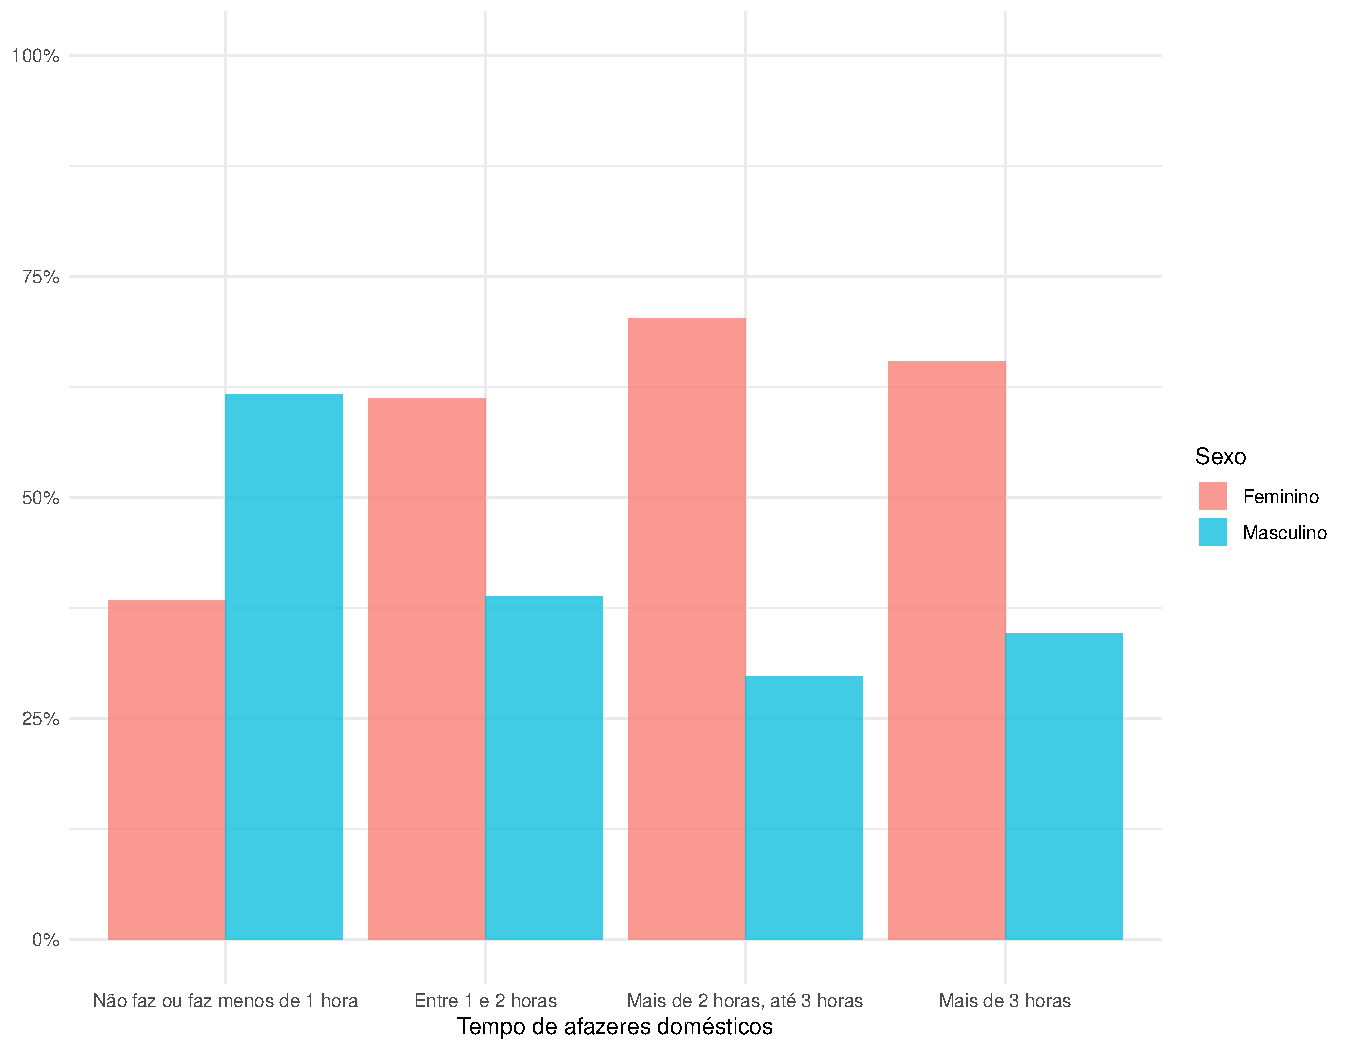
\includegraphics[width=16cm]{img/sexo_afazeres.pdf}
    \end{center}
    \fonte{Amostra de 5.271 alunos do 9\textsuperscript{o} ano do SAEB 2017.}
    \nota{Amostra retirada de uma amostragem aleatórias simples.}
\end{figure}


\newpage
Ao comparar os períodos de tempo nestes afazeres com o nível escolaridade da mãe (\autoref{esc_mae_afazeres}), a proporção de alunos que exercem estas atividades, para
cada nível escolar da  mãe, apresenta pelo menos 70\% localizado entre os que 
não fazem ou fazem até 2 horas.

%%%%% Gráfico de Escolaridade da mãe por afazeres_domesticos
\begin{figure}[h]
    \caption{Proporção total por nível de escolaridade da mãe
    com base no tempo de afazeres dos alunos.\label{esc_mae_afazeres}}
    \begin{center}
        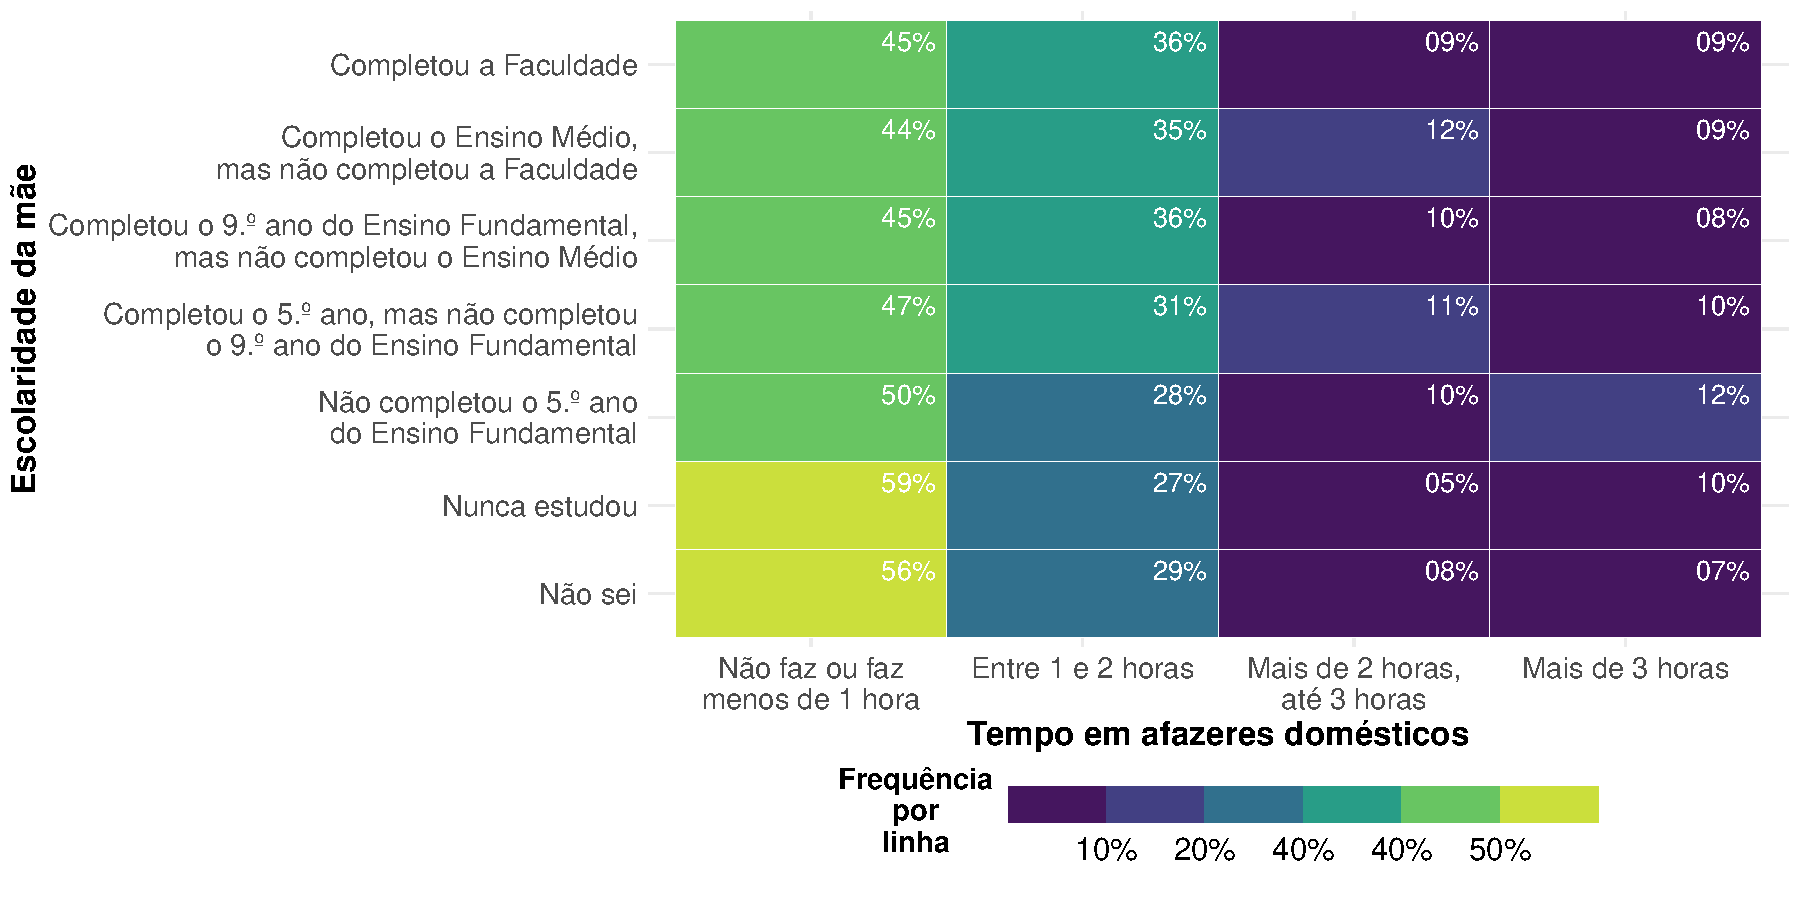
\includegraphics[width=16cm]{img/esc_mae_afazeres.pdf}
    \end{center}
    \fonte{Amostra de 5.271 alunos do 9\textsuperscript{o} ano do SAEB 2017.}
    \nota{Amostra retirada de uma amostragem aleatórias simples.}
\end{figure}

%%%%%%%%%%%%%%%%%%%%%%% Tabelas %%%%%%%%%%%%%%%%%%%%%%%%%%%%%%%%%%%%%%%%%%%%%%%%%%%%%%%%%%%%%%%%%

Ao realizar testes estatísticos com base nesses afazeres (\autoref{tab:af_test}) e com a
confiança de 95\%, a variável sexo obteve evidências significativas para afirmar que o tempo
médio não é igual entre os sexos, no qual o sexo feminino possui
proporções superiores em períodos de tempo maiores nestas atividades. Ao testar a variável
raça/cor dos alunos, não foram obtidas evidências significativas, apontando que não há indícios 
de diferenças, em média, entre as raças/cores, no tempo gasto nestes afazeres.
\clearpage
%%%%% Tabela dos testes paras relações com afazeres domesticos

\begin{table}[htb]
    \caption{Testes de igualdade na variabilidade sobre as relações 
            com o tempo de afazeres domésticos por parte dos alunos.}
            \label{tab:af_test}
        \centering
        \begin{tabular}{cccc}
        \toprule
        Teste & $H_0$& P-valor & Decisão de $H_0$ (95\%)\\
        \midrule \midrule
        K & $\mu_{Raça/Cor}$ iguais & 0.369 & Aceita\\
        K & $\mu_{Esc(mãe)}$ iguais & Aprox. 0 & Rejeita\\
        W & $\mu_M = \mu_F$ iguais & Aprox. 0 & Rejeita\\
        \bottomrule
        \end{tabular}
        \fonte{Amostra de 5.271 alunos do 9\textsuperscript{o} ano do SAEB 2017.}
        \nota{Amostra retirada de uma amostragem aleatória simples.}
        \nota[Anotações]{Os subíndices M e F referem-se, respectivamente, aos sexos Masculino e Feminino
        dos alunos. Esc (mãe) diz respeito à escolaridade da mãe destes. O Aprox. 0 refere-se a um número
        muito pequeno considerado por este estudo aproximadamente zero.}
\end{table}

O teste realizado com base na escolaridade da mãe sobre o tempo em afazeres domésticos,
ao mesmo nível de confiança, obteve evidências significativas sobre existência de diferença
no tempo gasto com afazeres domésticos. Ao efetuar testes pareados para cada nível escolar da mãe com a confiança
de 95\% (\autoref{tab:esc_mae_afzr}), a proporção de alunos que gastam tempo nestes
afazeres, para as mães que nunca estudaram se difere com todos os outros níveis escolares que,
em grande parte gastam menos de uma hora. O mesmo se observa para as mães com o
5\textsuperscript{o} ano incompleto, no qual o único grau que não se difere é dos alunos que
responderam que não sabiam sobre o nível educacional da mãe. As mães que completaram o 9\textsuperscript{o}
obtiveram igualdade apenas com as mães do 5\textsuperscript{o} ano, e aqueles que respoderam que não
sabiam. Para aquelas mães que completaram a faculdade, há igualdade entre as que completaram o
ensino médio, onde o tempo de afazeres por parte dos alunos para as mães com o nível de 
escolaridade do 5\textsuperscript{o} ano ou superior possui maiores proporções entre 1 e 2 horas
que entre as escolaridades abaixo desta.

\newpage
%%%%% Tabela de comparação da escolaridade da mãe com afazeres domesticos
\begin{table}[htb]
    \centering
\caption{Comparações dois a dois entre as ordens das posições sobre os tempos de afazeres domésticos
com base na escolaridade das mães dos alunos.\label{tab:esc_mae_afzr}}
    \begin{tabular}{lcc}
    \toprule
    Comparações & P-valor & Evidência (RA 95\%)\\
    \midrule \midrule
    Não sabe = Nunca estudou & Aprox. 0 & Desiguais\\
    Não sabe = Incompleto 5.\textsuperscript{o} ano do EF  & 1.0000 & Iguais\\
    Não sabe = Completou 5.\textsuperscript{o} ano do EF  & 0.0084 & Desiguais\\
    Não sabe = Completou 9.\textsuperscript{o} ano do EF  & 0.1927 & Iguais\\
    Não sabe = Completou EM & Aprox. 0 & Desiguais\\
    Não sabe = Completou Faculdade & Aprox. 0 & Desiguais\\
    Nunca estudou = Incompleto 5.\textsuperscript{o} ano do EF  & 0.0038 & Desiguais\\
    Nunca estudou = Completou 5.\textsuperscript{o} ano do EF  & Aprox. 0 & Desiguais\\
    Nunca estudou = Completou 9.\textsuperscript{o} ano do EF  & Aprox. 0 & Desiguais\\
    Nunca estudou = Completou EM & Aprox. 0 & Desiguais\\
    Nunca estudou = Completou Faculdade & Aprox. 0 & Desiguais\\
    Incompleto 5.\textsuperscript{o} ano do EF = Completou 5.\textsuperscript{o} ano do EF  & 0.0002 & Desiguais\\
    Incompleto 5.\textsuperscript{o} ano do EF = Completou 9.\textsuperscript{o} ano do EF  & 0.0048 & Desiguais\\
    Incompleto 5.\textsuperscript{o} ano do EF = Completou EM & Aprox. 0 & Desiguais\\
    Incompleto 5.\textsuperscript{o} ano do EF = Completou Faculdade & Aprox. 0 & Desiguais\\
    Completo 5.\textsuperscript{o} ano do EF = Completou 9.\textsuperscript{o} ano do EF  & 1 & Iguais\\
    Completo 5.\textsuperscript{o} ano do EF = Completou EM & Aprox. 0 & Desiguais\\
    Completo 5.\textsuperscript{o} ano do EF = Completou Faculdade & Aprox. 0 & Desiguais\\
    Completo 9.\textsuperscript{o} ano do EF = Completou EM & Aprox. 0 & Desiguais\\
    Completo 9.\textsuperscript{o} ano do EF = Completou Faculdade & Aprox. 0 & Desiguais\\
    Completou EM = Completou Faculdade & 1.0000 & Iguais\\
    \bottomrule
    \end{tabular}
    \centering
    \fonte{Amostra de 5.271 alunos do 9\textsuperscript{o} ano do SAEB 2017.}
    \nota{Amostra retirada de uma amostragem aleatória simples.}
    \nota[Anotações]{Aprox. 0 refere-se à algum número muito pequeno considerando aproximadamente zero.}
\end{table}

\newpage
%%%%%%%%%%%%%%%%%%%%%%%%%%%%%%%%%%%%%%%%%%%%%%%%%%%%%%%%%%%%%%%%%%%%%%%%%%%%%%%%%%%%%%%%%%%%%%%%%%%%%%%%%%%
%%%%%%%%%%%%%%%%%%%%%%%%%%%%%%%%% NOTAS %%%%%%%%%%%%%%%%%%%%%%%%%%%%%%%%%%%%%%%%%%%%%%%%%%%%%%%%%%%%%%%%%%%%%%%%%
%%%%%%%%%%%%%%%%%%%%%%%%%%%%%%%%%%%%%%%%%%%%%%%%%%%%%%%%%%%%%%%%%%%%%%%%%%%%%%%%%%%%%%%%%%%%%%%%%%%%%%%%%%%
\section{Notas}


%%%%%%%%%%%%%%%%%%%%%%% Graficos %%%%%%%%%%%%%%%%%%%%%%%%%%%%%%%%%%%%%%%%%%%%%%%%%%%%%%%%%%%%%%%%%
\newpage
%%%%% Grafico com raca cor e notas
\begin{figure}[h]
    \caption{Distribuições das somas das notas com base na raça/cor dos alunos.}
    \begin{center}
        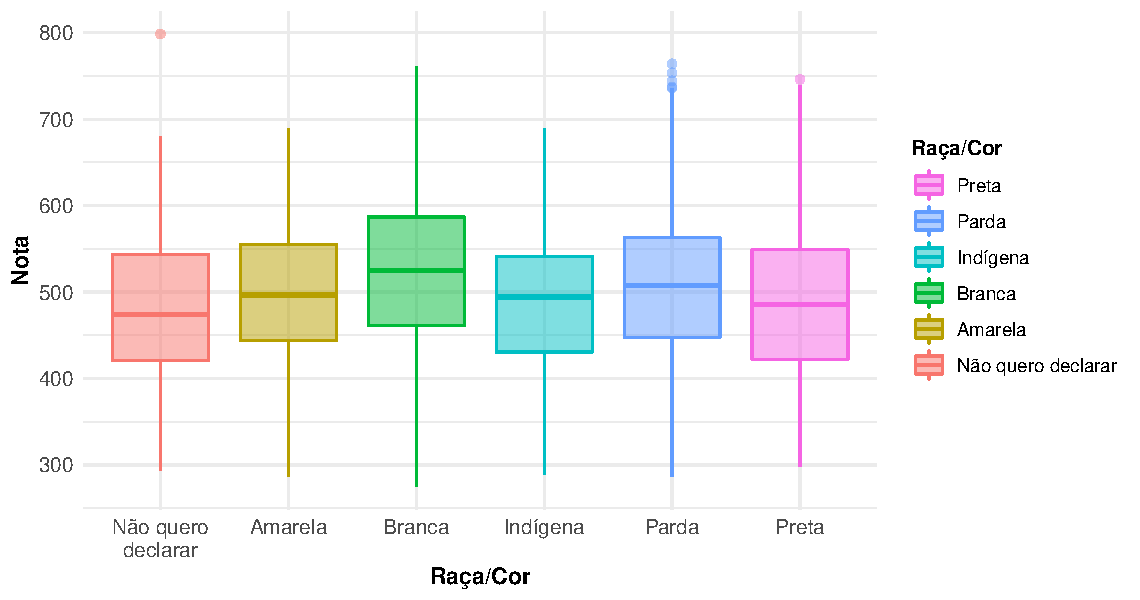
\includegraphics[width=16cm]{img/raca_cor_notas.pdf}
    \end{center}
    \fonte{Amostra de 5.271 alunos do 9\textsuperscript{o} ano do SAEB 2017.}
    \nota{Amostra retirada de uma amostragem aleatórias simples.}
\end{figure}


\newpage
%%%% Grafico localizacao com notas
A \autoref{img:loc_notas} mostra as distribuições das somas das notas por localização.
\begin{figure}[htb]
    \caption{Distribuições empíricas das somas das notas com base nas localizações das
    das escolas dos alunos.\label{img:loc_notas}}
    \begin{center}
        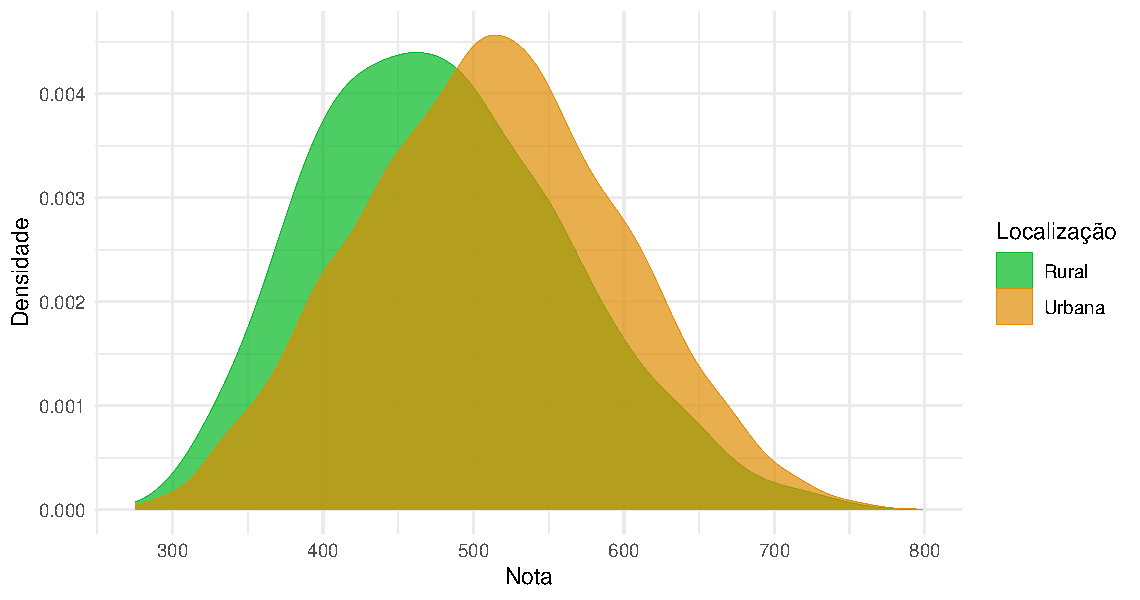
\includegraphics[width=16cm]{img/loc_notas.pdf}
    \end{center}
    \fonte{Amostra de 5.271 alunos do 9\textsuperscript{o} ano do SAEB 2017.}
    \nota{Amostra retirada de uma amostragem aleatórias simples.}
\end{figure}

É possível observar um grau de assimetria um pouco maior nas notas para a região rural
em relação à região urbana. A zona rural teve sua distribuição um pouco mais inclinada
para a esquerda, enquanto a zona urbana foi mais centralizada. É possível observar que
a moda das notas foi inferior na região rural em relação à região urbana.

A área rural apresentou uma nota média de 479, que também é inferior à nota média da
área urbana, que foi de 512.

\newpage
%%%%% Grafico da escolaridade da mae com notas
A Figura \ref{img:esc_mae_notas} mostra a distribuição das notas em relação à escolaridade
das mães.
\begin{figure}[h]
    \caption{Distribuições das somas das notas com base nas escolaridades 
    das mães dos alunos.}
    \begin{center}
        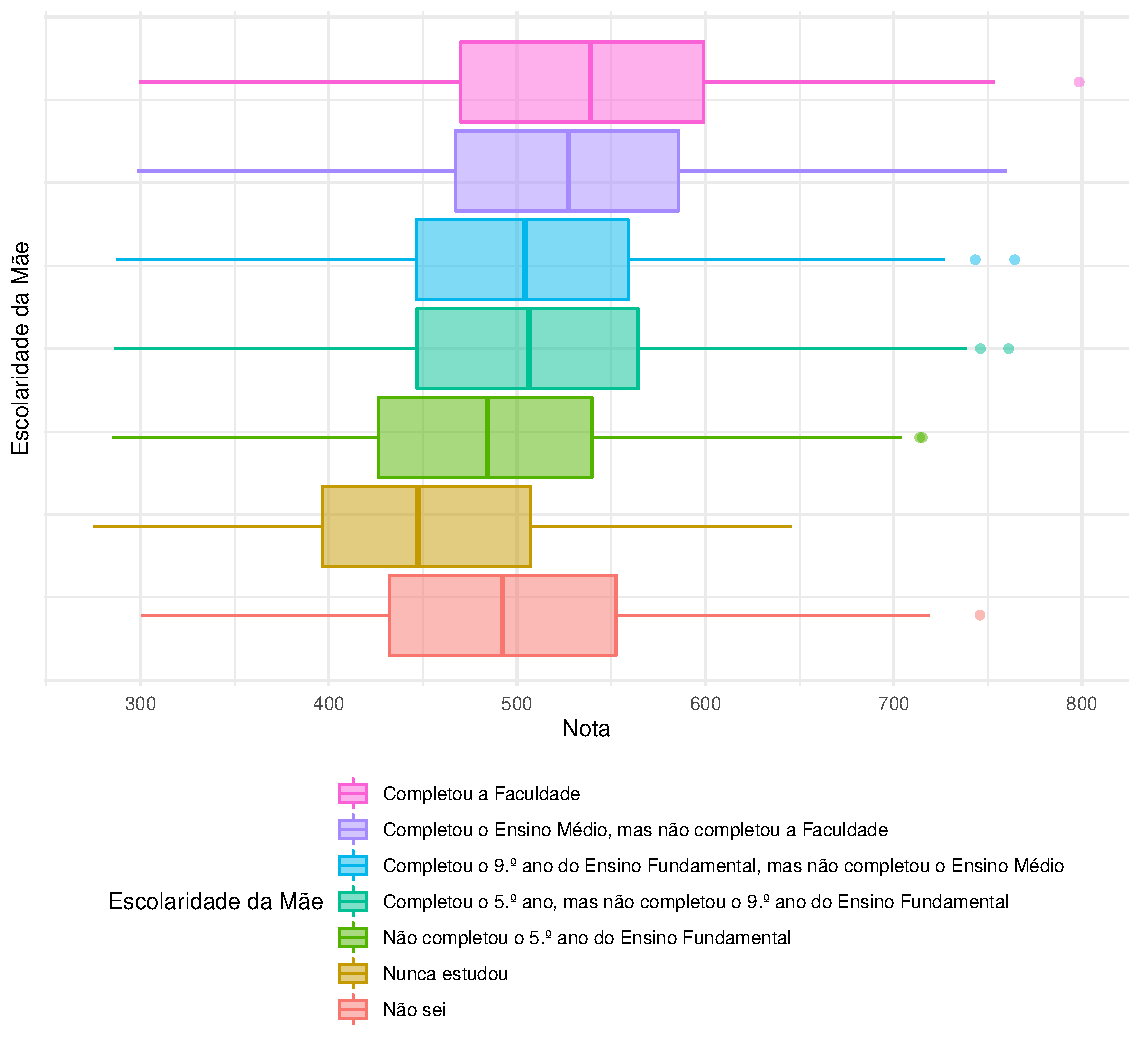
\includegraphics[width=16cm]{img/esc_mae_notas.pdf}
    \end{center}
    \fonte{Amostra de 5.271 alunos do 9\textsuperscript{o} ano do SAEB 2017.}
    \nota{Amostra retirada de uma amostragem aleatórias simples.}
    \label{img:esc_mae_notas}
\end{figure}

É possível observar um crescimento das notas no geral à medida que o grau de escolaridade
das mães é maior, de modo que filhos cujas mães têm grau de escolaridade alto têm tendência
a terem melhor desempenho em provas. Esse comportamento é observado mesmo entre os outliers,
onde a maior nota registrada vem da parte de um aluno cuja mãe completou a faculdade.



%%%%%%%%%%%%%%%%%%%%%%% Tabelas %%%%%%%%%%%%%%%%%%%%%%%%%%%%%%%%%%%%%%%%%%%%%%%%%%%%%%%%%%%%%%%%%
\newpage
%%%%%% Tabela com testes para as relacoes das notas
\begin{table}[htb]
\caption{Testes para as relações com soma
 das notas dos alunos.}
    \centering
    \begin{tabular}{cccc}
    \toprule
    Teste & $H_0$& P-valor & Decisão de $H_0$ (95\%)\\
    \midrule \midrule
    B & $\sigma_R^2 = \sigma_U^2$ & 0.503 & Aceita\\
    B & $\sigma_M^2 = \sigma_F^2$ & 0.002 & Rejeita\\
    B & $\sigma_{Raça/Cor}^2$ iguais & 0.265 & Aceita\\
    B & $\sigma_{Esc(mãe)}^2$ iguais & 0.132 & Aceita\\
    T & $\mu_R = \mu_U$ & Aprox. 0 & Rejeita\\
    T & $\mu_M = \mu_F$ & 0.905 & Aceita\\
    ANOVA & $\mu_{Raça/Cor}$ iguais & Aprox. 0 & Rejeita\\
    ANOVA & $\mu_{Esc(mãe)}$ iguais & Aprox. 0 & Rejeita\\
    \bottomrule
    \end{tabular}
    \fonte{Amostra de 5.271 alunos do 9\textsuperscript{o} ano do SAEB 2017.}
    \nota{Amostra retirada de uma amostragem aleatória simples.}
    \nota[Anotações]{Os subíndices, com base nos alunos, $R$ e $U$ refere-se as localizações
                    das escolas rurais e urbanas, M e F sobre os sexos Masculino e Feminino
                    respectivamente e Esc(mãe) diz respeito a escolaridade da mãe. 
                    O Aprox. 0 refere-se à algum número 
                    muito pequeno considerado por este estudo aproximadamente zero.}
\end{table}

\newpage
%%%%%% Tabela de comparacao entre raca/cor e notas
\begin{table}[htb]
    \centering
\caption{Comparações dois a dois entre as médias sobre a soma das notas
        com base na raça/cor dos alunos.}
    \begin{tabular}{lcc}
    \toprule
    Comparações & P-valor & Evidência (RA 95\%)\\
    \midrule \midrule
    Amarela = Não quero declarar & 0.4113 & Iguais\\
    Amarela = Branca & 0.0005 & Desiguais\\
    Amarela = Indígena & 1.0000 & Iguais\\
    Amarela = Parda & 1.0000 & Iguais\\
    Amarela = Preta & 1.0000 & Iguais\\
    Branca = Não quero declarar & Aprox. 0 & Desiguais\\
    Branca = Indígena & 0.0010 & Desiguais\\
    Branca = Parda & Aprox. 0 & Desiguais\\
    Branca = Preta & Aprox. 0 & Desiguais\\
    Indígena = Não quero declarar & 1.0000 & Iguais\\
    Indígena = Parda & 0.7758 & Iguais\\
    Indígena = Preta & 1.0000  & Iguais\\
    Parda = Não quero declarar & Aprox. 0 & Desiguais\\
    Parda = Preta & Aprox. 0 & Desiguais\\
    \bottomrule
    \end{tabular}
    \centering
    \fonte{Amostra de 5.271 alunos do 9\textsuperscript{o} ano do SAEB 2017.}
    \nota{Amostra retirada de uma amostragem aleatória simples.}
    \nota[Anotações]{Aprox. 0 refere-se à algum número muito pequeno considerando aproximadamente zero.}
    
\end{table}


\newpage
%%%%% Tabela de comparação da notas com Escolaridade da mae
\begin{table}[htb]
    \centering
\caption{\label{comp_MT}Comparações entre as médias de notas em Matemática e as regiões das escolas dos alunos com base na amostra de tamanho 500.}
    \begin{tabular}{lcc}
    \toprule
    Comparações & P-valor & Evidência (RA 95\%)\\
    \midrule \midrule
    Não sabe = Nunca estudou & 1.0000 & Iguais\\
    Não sabe = Incompleto 5.\textsuperscript{o} ano do EF  & 0.0078 & Desiguais\\
    Não sabe = Completou 5.\textsuperscript{o} ano do EF  & 0.0005 & Desiguais\\
    Não sabe = Completou 9.\textsuperscript{o} ano do EF  & 0.0001 & Desiguais\\
    Não sabe = Completou EM & Aprox. 0 & Desiguais\\
    Não sabe = Completou Faculdade & 0.0011 & Desiguais\\
    Nunca estudou = Incompleto 5.\textsuperscript{o} ano do EF  & 1.0000 & Iguais\\
    Nunca estudou = Completou 5.\textsuperscript{o} ano do EF  & 0.5598 & Iguais\\
    Nunca estudou = Completou 9.\textsuperscript{o} ano do EF  & 0.4165 & Iguais\\
    Nunca estudou = Completou EM & 0.1114 & Iguais\\
    Nunca estudou = Completou Faculdade & 0.4707 & Iguais\\
    Incompleto 5.\textsuperscript{o} ano do EF = Completou 5.\textsuperscript{o} ano do EF  & 1.0000 & Iguais\\
    Incompleto 5.\textsuperscript{o} ano do EF = Completou 9.\textsuperscript{o} ano do EF  & 1.0000 & Iguais\\
    Incompleto 5.\textsuperscript{o} ano do EF = Completou EM & 1.0000 & Iguais\\
    Incompleto 5.\textsuperscript{o} ano do EF = Completou Faculdade & 1.0000 & Iguais\\
    Completo 5.\textsuperscript{o} ano do EF = Completou 9.\textsuperscript{o} ano do EF  & 1.0000 & Iguais\\
    Completo 5.\textsuperscript{o} ano do EF = Completou EM & 1.0000 & Iguais\\
    Completo 5.\textsuperscript{o} ano do EF = Completou Faculdade & 1.0000 & Iguais\\
    Completo 9.\textsuperscript{o} ano do EF = Completou EM & 1.0000 & Iguais\\
    Completo 9.\textsuperscript{o} ano do EF = Completou Faculdade & 1.0000 & Iguais\\
    Completou EM = Completou Faculdade & 1.0000 & Iguais\\
    \bottomrule
    \end{tabular}
    \centering
    \fonte{Amostra de 5.271 alunos do 9\textsuperscript{o} ano do SAEB 2017.}
    \nota{Amostra retirada de uma amostragem aleatória simples.}
    \nota[Anotações]{Aprox. 0 refere-se à algum número muito pequeno considerando aproximadamente zero.}
    
\end{table}
